
\chapter{Network Security}%
\label{cha:Network Security}

From all of what we have done before, we assumed that the communication between Bob and Alice was a straight tube directly connected to our endpoints. But this is very far from reality, as seen in computer system, network is a much more complex infrastructure. Messages between Bob and Alice are converted into packets that are routed across \important{routers}, first in their \important{Local Area Networks (LAN)}, and then between networks (using \important{Wide Area Networks, WAN} protocols)
\begin{center}
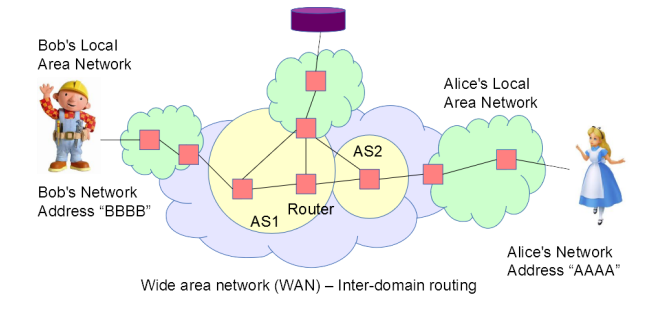
\includegraphics[scale=0.4]{screenshots/2026-11-26.png}
\end{center}
Router between local area networks are organized in \important{Autonomous System (AS)}, which follow a unique routing policy. Each AS is typically owned by one entity (e.g., and \important{Internet Service Provider, ISP}). From this network we would want to ensure some properties in order for Alice to send \important{securely} a message to Bob we want
\begin{itemize}
    \item \important{Naming Security}: We want to know the address of the receiver. Humans cannot remember machine-readable addresses; and also machine-readable addresses change over time. Thus we need Naming services to map high-level names to low-level names. It is important that we can grant the security of this naming servers. They must
		\begin{itemize}
		    \item \important{Integrity}: the (name, address) association must not be modified by unauthorized entities
		    \item \important{Authentication}: users need to be able to verify that the (name, address) association come from an authoritative source (i.e., a source entitled to set this association)
		    \item \important{Availability}: the naming service must be available to grant service to users
		\end{itemize}
    \item \important{Routing security} It is important that the route over the network and the eventual delivery of messages must not be influenced by the adversary. This implies
		\begin{itemize}
		    \item \important{Integrity}: of the route must not be modified by unauthorized parties
		    \item The route must only go through the chosen routers, thus the identity of the routers must be authentic
		    \item The route (and the routers therein) must be available to route packets
		\end{itemize}
    \item All messages/packets within a session must arrive to the receiver without modification, in order or number (i.e., no messages can be added or removed). The integrity of the messages must be maintained and they must come from authentic source
    \item The content must not be influenced (its integrity must be protected), and many times not readable (i.e., we need confidentiality), by non-authorized parties.
\end{itemize}
In this course we will ask the following questions
\begin{itemize}
    \item Do deployed network protocols provide the desired properties? That is those the naming, routing, session, content security hold the previous properties?
    \item What are the existing solutions to improve network security?
\end{itemize}
As said previously, computers communicate with each other at different layers. These are typically modeled by the Open System Interconnection (OSI) Model. This model covers from the physical layer, where pulses that codify bits are sent, to the application layer where programs talk to each other. In this section we will cover protocols at different layers, and see the security problems and potential solution

\section{ARP Spoofing}
Let us first have a little refresh on routing. What do we mean by routing IP on an ethernet LAN. A Lan is a network that spans a (typically) small geographic area, and connect devices that are local in this area. Inside the LAN, these devices have two addresses:
\begin{itemize}
    \item Address at the link level: a unique address called the \important{MAC} address. Each machines have a '\textit{unique}' 48 bits MAC (Media Access Control) address
    \item Address at the network level: the \important{IP} address, each machine has an IP address which is 4 bytes in IPv4
\end{itemize}
\begin{parag}{How does IP routing work?}
    To route a IP packet, Alice needs to know her own address, and Bob's address. Furthermore, Alice needs to know her own subnet, which tells her on which LAN she and Bob are; and her gateway which she needs to use to communicate with Bob if he is not on the same subnet. First, Alice checks if she and Bob are on the same subnet by using the mask. If they are, Alice needs Bob's MAC address to route his mesage. If they are not, Alice needs the MAC address of the gateway to route her message out of the LAN.
\end{parag}
\begin{parag}{And inside the LAN?}
    If we are inside the LAN then it is our job to find Bob's MAC address. To do so we use \important{ARP (Address Resolution Protocol)} which enables machines to find mappings between IPs and MACs inside. How this essentially work is by Alice first storing a cache of mappings between IP addresses and MAC addresses. If Bob's IP address is not in her cache, she will broadcast an ARP request to look for his IP address.
\end{parag}
\begin{parag}{Is it safe?}
    Now recall the property of naming security: \textit{The association between lower level names (e.g. network addresses) and higher level names (e.g. Alice/Bob)} must not be influenced by the adversary. Does ARP provide naming security? Recall that ARP is a '\textit{translation}' between IP address and MAC address
	\begin{itemize}
	    \item Each host maintains a cached table of $IP \iff MAC$ mappings
	    \item If it is not available, the host \important{broadcast} an ARP request to query for target IP
	    \item An ARP reply responds with the MAC address for that IP
	\end{itemize}
	The packet format in which does are sent \important{does not include signature nor message authentication code}
	\begin{center}
	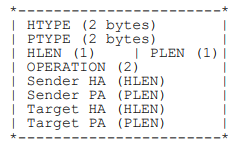
\includegraphics[scale=0.4]{screenshots/2026-11-26_1.png}
	\end{center}
	Therefore the receiver cannot check the \important{integrity} of the packet and the \important{authenticity} of the sender! But if nobody checks, this mean that you can \important{impersonate} and provide the identity of others. The modification of ARP packets by changing the content or impersonating other computer is called \important{ARP spoofing}. What we can achieve here are a lot of bad stuff,
	\begin{itemize}
	    \item Impersonation (this is bad...)
	    \item Man in the middle: provide two hosts (sender/receiver) with your MAC address and monitor communication or tamper with it
	    \item Abuse resource allocation
	    \item Deny service to a machine in the network. This could be done by launching a MITM attack and not relying messages, or by just ensuring that any ARP request to the victim of the attack is always responded with a wrong MAC address. This way, no sender will find the correct mapping (IP,MAC) for the victim and the victim cannot receive messages.
	\end{itemize}
	The possibility to impersonate other computers in the network also enables adversaries to steal resources allocated to others. For instance imagine a LAN in which bandwidth is limited per MAC address. By spoofing others' address you can enjoy more bandwidth than initially allowed. This is also bad for routing security. But notice that the same happens in DNS, IP, Ethernet, ... No network protocol was (initially) designed with security in mind! The reason for this was the thread model used when designing those. The thread model was that outsiders are bad, insiders behave, trust them! Which indeed sounds like an awful idea.
\end{parag}
\begin{parag}{ARP spoofing - Defenses}
    The problem of ARP soofing is rooted on the that that there is no authentication of who is providing a mapping IP $\iff$ MAC.\\
	One solution would be to not ask in the network (where spoofing is possible) but to ask in an out of band channel, e.g. asking in person where authentication is easy. Then one can store the learned mappings on a static real-only mapping. While this is a very secure means: authentication is granted, it does not scale and it is not flexible: everytime there is a change in an association one needs to manually learn the new mapping and update the table. Thus, this is typically only used for critical services whose failure may have big repercussions. For instance, to secure the mapping IP $\iff$ MAC for the gateway.\\
	For the other case, one can prevent spoofing by
	\begin{itemize}
	    \item Instead of taking the first IP $\iff$ MAC association returned by ARP as truthful, one can check whether there is an inconsistency: there is ore than one IP associated to this MAC in your cache table, there is an IP for which you have seen more than one MAC, you observer packets with morethan one MAC associated to the IP.
	    \item Instead of taking the first IP $\iff$ MAC association returned by ARP as truthful, ask other members of the network if they have the same observation, i.e., cross-check the discovery.
	    \item Send an email to the user, or the system administrator, if one observes a change in an IP $\iff$ MAC association. Only validate the change if a person confirms it is correct.
	\end{itemize}
	Note that the two last methods effectively implement the concept of separation of privilege by requiring that the adversary compromises more than one entity (more than one machine in the network in the first case, and one human in the second case).
\end{parag}

\section{DNS Spoofing}
\begin{parag}{Refresher of Domain Name Service (DNS)}
    In order to resolve a domain, a client send a DNS query to a \textit{recursive} resolver (I think it can also be a iterative one (from CS-202)), a server typically provided by the ISP with resolving and caching capabilities. If the domain resolution by a client is not cached by the recursive name server, it contacts Root Server, Top Level Domain server, and then authoritative name server which hold a distributed database of domain names to IP mappings. The recursive resovler traverses the hierarchy of authoritative name servers until it obtains an answer for the query, and sends it back to the client. The client can use the resolved IP address to connect to the destination host.
\end{parag}
\begin{parag}{Attacks}
    As in the ARP protocol, DNS request and responses do not include any kind of security protection. Two attacks are possible
	\begin{subparag}{Cache poisoning}
	    This attack exploits the fact that resolvers do not authenticate the origin of a response to include an association (domain name, IP). Therefore, an adversary can introduce fake associations to direct users visiting target domains to IPs controlled by the adversary.
	\end{subparag}
	\begin{subparag}{DNS Hijacking}
	    This attack exploits the fact that responses do not have authenticity or integrity protections. The adversary intercepts the response from the resolver, and modifies the IP in the response to an IP that she controls, in order to direct the vitctim to a machine she controls.
	\end{subparag}
	But one can get other bad studd to happen, what can cause Denial of Service, by avoiding that packets arrive to one host $\to$ censorship. One can also achieve redirection; we can reroute clients to malicous host which can either directly attack the client (e.g. serving malware) or by the malicious host acting as a man in the middle (e.g., monitoring)
\end{parag}
\begin{parag}{Defenses}
    As always, the attacks exploit the fact that there is no protection of the associations or the responses. A first attempt to protect DNS is DNSSEC, which stands for Domain Name System Security Extension (not very creative...). We can introduce extension to DNS that provide origin authentication by having
	\begin{itemize}
	    \item DNS responses that are digitally signed by authoritative name server which prevents poinsoning!
	\end{itemize}
	A major problem with DNS is that, even if the integrity and the authenticity of the responses are maintained, as those are not encrypted and adversary observing the communication can still monitor the users' actions. For this reason nowadays new protocol encrypt DNS, e.g. by tunneling requests and responses into an HTTPS or TLS connection, which provide all authenticity, integrity and confidentiality as we see later in the section.
\end{parag}

\subsection{BGP Spoofing}
Okay we have DNS fixed but is this enough? In this case those the routing security which was that \textit{the route over the network and the eventual delivery of messages must not be influenced by the adversary} is maintained? Let us first recall that BGP (Border Gateway Protocol). We have seen that inside AS we are good we have seen how it works? how to make it secure etc. But what happens between AS (Autonomous System). BPG constructs the routing tables between AS with independent routing domains. We have
\begin{itemize}
    \item Routers maintain tables of (IP subnet $\to$ Router IP, cost)
    \item Routes change (faults, new contracts, new cables); Implying that BPG needs to be updated constantly
    \item The Cost is \important{crucial}: BGP chooses the routes with lowest cost (real money)
\end{itemize}
\begin{framedremark}
Here are a link for the course on more details on the protocol
\begin{center}
https://blog.cdemi.io/beginners-guide-tounderstanding-bgp/
\end{center}
\end{framedremark}
\begin{parag}{BGP Security}
    BGP provides some authentication mechanics, that enables routers to now that they are talking with other routers. The mechanism is very basic: uses a short secret and a broken hash algorithm. Even if this mechanism would be secure, it only makes sure that routers speak with other routers, but does not provide any assurance on the information the routers provide. Thus, an adversary controlling a router can advertise any route they want, advertisement will propagate to other routers. As in the previous cases, by rerouting traffic,the adversary can monitor or deny service.
	\begin{subparag}{Remark}
	    Note that this attack in itself does not enable the adversary to redirect traffic to their own server (as ARP spoofing or DNS spoofing do). The attack allows the adversary to only modify the route, not the destination. If the adversary then can run an on-path attack, and modify packets, then they can run an IP-spoofing attack or other means to redirect.
	\end{subparag}
	\begin{subparag}{Example: Belarus hijacks internet}
	    Global traffic has been redirected to Belarusian ISP GlobalOneBel.
		\begin{itemize}
		    \item Daily basis throughout February 2013
		    \item Changing set of victims: major financial institutions, governments, and network service providers
		    \item Affected countries included the US, South Korea, Germany, the Czech Republic, Lithuania, Libya, and Iran
		\end{itemize}
	\end{subparag}
\end{parag}
\begin{parag}{BGP Spoofing Defenses}
    A possible defense would be, as in ARP to try to identify inconsitencies in the routes. A packet traveling from Switzerland to Italy should not need to go through the US. Yet there is no real definition for \textit{'correct route'} as routes do also depend on economical factors. There is a standard BGPSec, that is similar to DNSSec which aims at mitigating hijacking but ensuring that routers are signed by authoritative ASes, i.e., those hosting the IPs.
\end{parag}

\paragraph{Spoofing: lesson to be learned}%
\label{par:Spoofing: lesson to be learned}
\begin{parag}{1. The network is hostile}
    Routing security attacks, faciliated through \important{poor association of high level and low level names and addresses (IP to Ethernet MAC/ Route to router)}. Threat model assuming that network insiders are trusted to provide authoritative information lead to a whole suite of protocols being susceptible to attacks that endanger Internet transactions.
\end{parag}
\begin{parag}{2. The solution is intimately linked to cryptography}
    As there is no TCB that can enforce a policy, most of the solutions rely on cryptography to ensure integrity, authentication and confidentiality. Yet, cryptographic solutions fall short in some cases as they still rely on a given definition of authority (e.g., authority to provide a BGP route, authority to provide a domain-IP mapping). How to define these authorities is not a security problem, but a policy one.
\end{parag}

\section{IP Spoofing}
As said before, computers communicate with each other at different layers. These are typically modeled by the Open system Interconnection (OSI) Model. This model covers from the physical layer, where pulses that codify bits are sent, to the application layer where programs talk to each other. In this lecture we will cover protocols at different layers, and see the security problems and potential solutions.  We have seen the ARP routing, DNS and BGP which all are below or at the Network level. But what IP? The Internet Protocol (IP) enables addressing and routing of packets between hosts in a network. For the purpose of this lecture, the most important factor is that IP packets, as all the other protocols do not include any protection (just a non-cryptographic checksum to detect transmission errors) to preserve the integrity of the source and destination address, not the integrity and confidentiality of the data. This again enable adversaries to tamper with the IPs (IP spoofing) and learn the destination of packets (privacy invasion). By being able to spoof source IPs we can achieve: 
\begin{itemize}
    \item \important{Impersonation}: we can fake being others. This could be useful to take advantage of others' resources, for instance in networks that allocate resources based on IP.
    \item \important{Man in the Middle}: if we can impersonate others, we can launch a man-in-the-middle attack and monitor, change or deny communication. Note that for a min in the middle we may need to also hijack the TCP connection to achieve a link between MAC and IP
    \item \important{Denial of Service}: we can use spoofing to trigger the sending of packets from e.g., a server, to a victim computer. This is done by telling that server that packets originate from the victim's computer IP.
\end{itemize}

To resolve this let us introduce \important{IPSec} which stands for Internet Protocol Security. We now complements the IP with cryptographic security properties directly at the IP level. We first exchange key based on a public key cryptography or symmetric key and then provide two protocols:
\begin{parag}{Authentication Header protocol (AH)}
    It provides a mechanism for header authentication only. AH provides data integrity, data origin authentication, and, optionally, replay protection. Data integrity is ensured by including a digest generated by a secure message authentication algorithm such as HMAC-SHA. Data origin authentication stems from the use of a shared secret key (remember from the cryptography lecture that this provides authentication for the communication parties, but not repudiation against third parties). Replay protection relies on a sequence number field with the AH header. AH authenticates IP headers and their payloads, with the exception of certain header fields that can be legitimately changed in transit, such as the Time To Live (TTL) field. AH does not provide confidentiality of content. Also AH breaks NAT, why?
\end{parag}


\begin{parag}{Encapsulating Security Payload protocols (ESP)}
    It provides data confidentiality (encryption) and authentication (data integrity, data origin authentication, and replay protection). It can be configured to provide only confidentiality, only authentication, or both. When ESP provides authentication functions, it uses the same algorithms as AH, but protects different parts. AH authenticates the entire IP packet, including the outer IP header, while ESP only authenticates the IP datagram portion of the IP packet.\\

	ESP+Null can be sort of used to avoid spoofing. You lose the strict "\textit{Anti-Spoofing}" protection on the IP header itself. You are trusting that if the data inside is signed correctly by the sender, the packet probably came from them, even if the IP header was modified by a router along the way.
\end{parag}

These two protocols can be used in two modes:
\begin{itemize}
    \item \important{Transport mode}: it protects the packet payload (authentication and/or confidentiality depending on the choice). The origin IP header is left intact. This means that the original information, such as origin and destination, are still available and observable.
		\begin{center}
		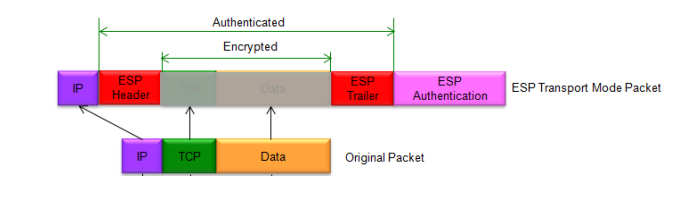
\includegraphics[scale=0.4]{screenshots/2026-11-26_2.png}
		\end{center}
    \item \important{Tunnel mode}: tunnel mode creates a \textit{new header}. The full packet is encrypted and authenticated. This way, the original source and destination of a packet are protected from potential observers.
		\begin{center}
		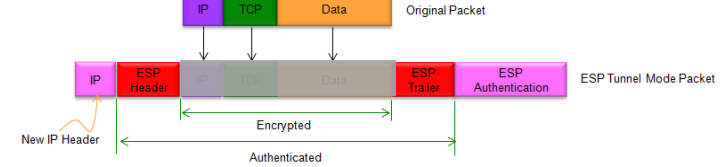
\includegraphics[scale=0.4]{screenshots/2026-11-26_3.png}
		\end{center}
\end{itemize}

\begin{parag}{Use of IPSec: Virtual Private Network}
    Using IPSec in tunel mode is one of the means to create \important{Virtual Private Network (VPN)}. A VPN is a private network that uses a public network (typically, the internet) to connect remote hosts. The VPN uses '\textit{virtual}' connections to route from one host to the other. Inside the VPN, routing is Local 
	\begin{center}
	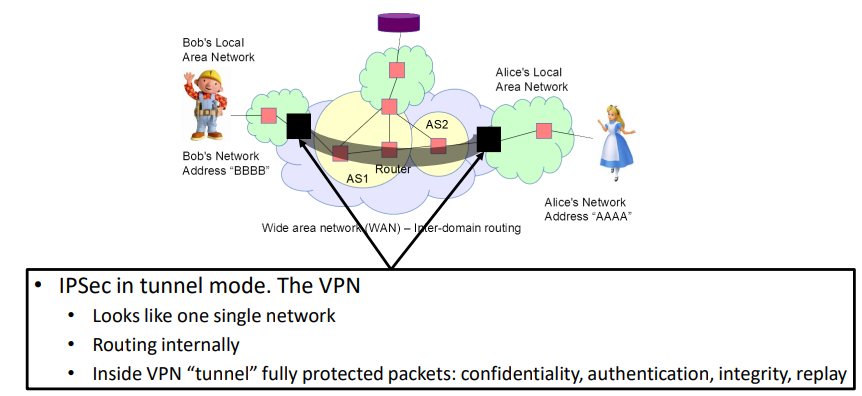
\includegraphics[scale=0.4]{screenshots/2026-11-26_4.png}
	\end{center}
	Here Bob can locally route to Alice using local routing. Inside the VPN tunnel, packets are fully protected by IPSec. When Bob wants to send a packet to Alice, instead of doing (simplified) 
	\begin{align*} 
		\left\{src_{IP}, dst_{IP}, Data\right\} = \left\{IP_{Bob}, IP_{Alice}, Data\right\}
	\end{align*}
	Bob prepares an encapsulated packet such that 
	\begin{align*} 
		\left\{IP_{Bob}, IP_{VPN}, Enc\left(IP_{Bob}, IP_{Alice}, Data\right)\right\}
	\end{align*}
	This packet is sent to the entry of the VPN that transmits it to the exit. The exit decrypts the packet and then can send it to Alice. In transit, an adversary between Bob and the entry to the VPN cannot see the destination  or the payload. An adversary between the entry and the exit to the VPN cannot see the origin, the destination or the payload.
\end{parag} 
However even if VPNs provide confidentiality, authentication, integrity, and reply protection for the packets. It still does not protect any higher layer: authentication problems at the application layer, or denial of service problems cannot be solved with IPSec.

\begin{parag}{Virtual Private Network as a Service}
    VPNs do not necessarily need to join two local networks. They can be used to simply leave the local network from another exit point than the gateway. This is the typical use of a VPN to change one's IP (e.g., to user pay TV services on another country).\\
	
	Notice also that rewriting/hiding 
\end{parag}


your IP isn't just a privacy feature of a VPN, it is necessary for the VPN to work/ Think of an IP address like a return address on an enveloppe.
\begin{itemize}
    \item \important{without the VPN}: you send a letter to Google. You write your return address on it. Google reads the letter and mails the reply directly to you.
    \item \important{With VPN}: you put your letter inside a secure, steel box (the encrypted tunnel) and ship it to the VPN company.
		\begin{itemize}
		\item The VPN company opens the box.
		\item They take out your letter
		\item \important{Crucial step}: If they mailed your letter to Google with your return address still on it, Google would mail the reply directly to your house. This would break the security/encryption.
		\item \important{The fix}: the VPN company crosses out your return address and writes \important{their own} return address.
		\item Now, Google mails the reply to the VPN company. The VPN company puts it back in the steel boc and ships it to you
		\end{itemize}
\end{itemize}



\begin{parag}{Is a VPN the same as a proxy}
    Even the last use of a VPN may remind us of a proxy, a proxy and VPN provide very different security properties. They do not protect users in the same threat model. Proxies are at the boundary between two networks, and rely traffic from one network to the other. In a way, they act as man in the middle and can see what happens in both sides. The traffic is not encrypted end to end, but only end-ro-proxy.\\
	$ $\\
 	A VPN creates one network! The traffic is encrypted end-to-end. There is no middleman that can see what happens in both side.
\end{parag}






\section{TCP}
The goal of IP is to facilitate routing, but it does not feature many other desirable properties to have reliable, robust, efficient communications. Those are provided at the transport layer by the \important{Transmission Control Protocol (TCP)}  that runs just above IP in the OSI model. TCP helps establishing and maintaining a connection to exchange a stream of messages. It determines how the data set by the application is divided into packets that can be routed through the network. It manages flows, retransmission, and order. For the purpose of this section we care about
\begin{itemize}
    \item Ports: these are used to multiplex applications over a connection.
    \item Sequence, window, and acknowledgement numbers: these are used to manage the flow number and guarantee error-free transmissions
    \item Flags: \texttt{ACK} (the packet is an acknowledgement), \texttt{RST} (terminate a connection), \texttt{SYN} (acknowledge the begin of a session), \texttt{FIN} (another way of terminating a connection)
\end{itemize}
\begin{center}
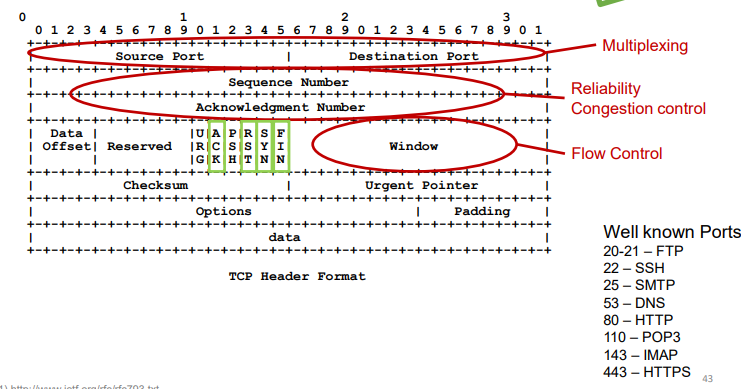
\includegraphics[scale=0.4]{screenshots/2026-11-27.png}
\end{center}

Recall also the TCP 3-way handshake where we have three steps

\begin{enumerate}
    \item \texttt{SYN}: in the first step, client declares the desire to establish a connection with the server using the \texttt{SYN} flag and sending a sequence number SecC with which it will start sending segments with
    \item \texttt{SYN + ACK}: the server responds with both \texttt{SYN-ACK} signal flags set. \texttt{ACK} responds the request of the  client (using the received sequence number increased by one unit, \texttt{SeqC + 1}), and \texttt{SYN} indicating which sequence number will the server use.
    \item \texttt{ACK}, Finally, the client acknowledges the response of server and they both establish a reliable connection with which they will start the actual data transfer.
\end{enumerate}
TCP, like the previous protocols does not include any integrity or authentication mechanism. The sequence number act as very weak secret that is used as authentication. Both client and server will accept packets as long as they have sequence numbers that correspond to the current session.
\begin{parag}{TCP 3-way handshake - Security considerations}
    The question that we are asking is whether an adversary could be able to have a reasonable guess on. The issue here is that if an adversary can guess the sequence numbers, the adversary can hijack the connection and deny service, man in the middle, etc. Therefore can it guess?
	\begin{itemize}
	    \item If the adversary is on path, the adversary can directly observe the sequence number and use this observation
	    \item In some cases, hosts use a weak random number generator (e.g., based on current time), that enables the adversary to make a good guess with high likelihood.
	\end{itemize}
	The Robert Morris attack exploits this, together with the fact that IP is easy to spoof to take over remote sessions opened using the '\textit{rsh}'
	
	\begin{subparag}{Robert MOrris Attack}
	    \begin{enumerate}
	        \item Send a \texttt{SYN} packet \important{spoofed} as if it was from authorized host
	        \item Guess server SeqS and send an \texttt{ACK} with \texttt{SeqS + 1} and some data
	        \item The data is interpreted as a shell command and executed!
	    \end{enumerate}
	    
	\end{subparag}
\end{parag}


\subsection{Transport Layer Security}
In the case of TCP, it is hard to add cryptographic operations to authenticate the exchange, as it was done with previous protocols. Seuciryt checks cannot only happen during the login phase (the establishment of the TCP connection). To apply the mediation principle, you would need per packet authentication. Every single piece of data sent must be cryptographically signed so the receiver knows it came from the real user, not an imposter injecting data into the stream. TCP cannot do that. Therefore, to solve this issue, a new '\textit{layer}' appeared between the TCP/IP level and the application. Here the \important{Transport Layer Security Protocol (TLS)}  provides the properties that TCP cannot :
\begin{itemize}
    \item Confidentiality: it enables hosts to agree on a symmetric key to encrypt their packets
    \item This key can be agreed in such a way that the protocol provides forward secrecy, i.e., if the adversary learns the key of one TLS session, this key does not enable the adversary to decrypt previous sessions.
    \item Authentication: it enable hosts (servers and clients) to use public key cryptography to authenticate themselves
    \item Integrity, through the use of signatures when using public key crypto, and MAC when using symmetric crypto.
\end{itemize}
Even though the state-of-the-art is TLS 1.3, there are many lower, insecure, versions of TLS (and even its predecessor SSL) are still deployed. This is because updating machines is hard. Many are badly managed, or managed with people with low security knowledge, or simply need to maintain the previous version to keep their operation.
\begin{parag}{TLS handshake}
    All the security properties provided by TLS are bottstrapped in the TLS handshake in which two hosts (e.g. client and server) agree on a key.
	\begin{subparag}{Step 1}
	    The client declares its willingness to start a secure TLS connection and informs the server of 
		\begin{itemize}
		    \item The higher TLS version it is able to speak
		    \item  The cipher suites (algorithms for key agreement, signature, encryption, and hashing) it can compute. This is a list of tuples such as the one in the example, ordered by the client preferences – in general from more secure to less secure.
		    \item  A session ID to identify the TLS flow
		    \item  A challenge to ensure freshness of the communication (i.e., reply prevention)
		\end{itemize}
	\end{subparag}
	\begin{subparag}{Step 2}

		the server declares its willingness to continue the secure TLS informs the
client of:
		\begin{itemize}
			\item From the cipher suites offered by the client, which one is preferred by the server.
			\item  The server certificate: a signature on the public key of the server by an authority trusted by the client. It enables the client to verify the identity of the server given a signature with the server’s private key.
			\item  If the client and server are agreeing on a key, e.g., using Diffie-Hellman, then the server provides material to derive the key (e.g., $g^{a}$).
			\item  Optionally, the server can also ask the client to provide a certificate for two-sided authentication.
			\item  A challenge to ensure freshness of the communication (i.e., reply prevention).
		\end{itemize}
	\end{subparag}
	\begin{subparag}{Step 3}
	    The client responds with:
		\begin{itemize}
			\item - If the server requests it: the client’s certificate: a signature on the public key of the client by an authority trusted by the server. It enables the server to verify the identity of the client given a signature with the client’s private key.
		\item  If the client and server are agreeing on a key, e.g., using Diffie-Hellman, then the client provides material to derive the key (e.g., $g^{b}$).
		\item  Sends a flag indicating that from then on the client will send all messages encrypted and authenticated using the algorithms agreed on Step 2 using the key derived on Step 3
		\end{itemize}
	\end{subparag}
	\begin{subparag}{Step 3.1}
	    The client informs the server that it has finished its side of the handshake. This message, as it follows the \texttt{ChangeCipherSec} flag, is already encrypted and authenticated.
	\end{subparag}
	\begin{subparag}{Step 4 and 4.1}
	    the server also indicates that it will, from then on, encrypt and authenticate all messages as agreed; and indicates that it has finished its side of the handshake.
	\end{subparag}
	TLS offers two modes to obtain a shared key between server and client:
	\begin{itemize}
	\item Key transport: using the public key of the server, the client sends a symmetric key. This mode is not forward secure, as if at any point the key of the server falls in the hand of an adversary, this adversary can decrypt all keys in the past.
	\item  Key agreement: using Diffie Hellman (or its Elliptic curve equivalent) the client and server agree on an ephemeral key for the session. This key is independent in every session.
	\end{itemize}
\end{parag}


\subsection{Denial of Service}
\begin{parag}{Example 1 -- Skype kittens DoS (CVE-2018-8546)}
    When receiving about 800 emoji of kittens at once, the Skype for Business client stopped responding for a few seconds. If a sender continues sending emojis, the client will not be usable until the attack ends.\\
	Improper handling of emojis in Microsoft Skype for Business and in Lync enables an adversary to \important{consume all the resources} associated to these programs in such a way that they cannot be used for any useful activity (calling, messaging, etc).
\end{parag}

\begin{parag}{Example 2 -- TCP SYN flood}
    Recall the TCP handshake: after receiving a SYN and sending a SYN/ACK, the server is listening, waiting for the next ACK in order to establish the connection. In the meantime it stores some information about the connection in a so-called \important{TCP Control Block (TCB)} ($\sim 280$ bytes).
	\begin{subparag}{How does the attack work?}
		\begin{itemize}
		    \item Send TCP SYN packets with bogus source address
		    \item Half-open TCB entries exist until timeout
		    \item The kernel limits the number of TCBs!
		\end{itemize}
		Resources exhausted $\Rightarrow$ new requests rejected. The adversary exhausts the space for TCBs, and then the host cannot open new connections anymore.
	\end{subparag}
\end{parag}

\begin{parag}{TCP SYN flood Prevention -- use ``cookies''}
    \important{Principle}: minimize the state before you are ``authenticated'' (i.e., before finishing the 3-way handshake). Don't create the full TCP Control Block, instead
	\begin{itemize}
	    \item \important{Compress TCP state}: very tiny state representation for half-open connections. A few bytes per connection $\Rightarrow$ can store 100,000s of half-open connections, orders of magnitude more than before.
	    \item \important{Push the state to the client!} (``SYN cookies''). The idea is to not store the TCB but to send it to the client:
			\begin{enumerate}
			    \item Upon receiving a message, derive the state
			    \item Cryptographically protect the state under a fixed key (confidentiality and integrity) $\to$ this is the cookie, the server does \textbf{NOT} store it
			    \item Send it back to the client: the server substitutes its sequence number $Seq_S$ by the cookie
			    \item Require the client to provide it back to complete the protocol: the server subtracts 1 from the received acknowledgment number ($Seq_S + 1$) and checks the validity of the cookie
			\end{enumerate}
			As the state is cryptographically protected, the server can check its correctness when it comes back.
	\end{itemize}
	\begin{subparag}{Remark}
	    Original SYN cookies explanation: \url{http://cr.yp.to/syncookies.html}
	\end{subparag}
\end{parag}

\begin{parag}{Other methods: Proof of Work}
    An ``economic'' measure to deter denial of service attacks: require the client to do some work before engaging in the operation (e.g., compute some hashes). This is easy to do once and to verify, but expensive to do many times, which is exactly what a DoS needs. It is not a perfect countermeasure, but it increases the cost barrier to deploy DoS at large scale.
\end{parag}

\begin{parag}{TCP header}
    \begin{verbatim}
 0                   1                   2                   3
 0 1 2 3 4 5 6 7 8 9 0 1 2 3 4 5 6 7 8 9 0 1 2 3 4 5 6 7 8 9 0 1
+-+-+-+-+-+-+-+-+-+-+-+-+-+-+-+-+-+-+-+-+-+-+-+-+-+-+-+-+-+-+-+-+
|          Source Port          |       Destination Port        |
+-+-+-+-+-+-+-+-+-+-+-+-+-+-+-+-+-+-+-+-+-+-+-+-+-+-+-+-+-+-+-+-+
|                        Sequence Number                        |
+-+-+-+-+-+-+-+-+-+-+-+-+-+-+-+-+-+-+-+-+-+-+-+-+-+-+-+-+-+-+-+-+
|                    Acknowledgment Number                      |
+-+-+-+-+-+-+-+-+-+-+-+-+-+-+-+-+-+-+-+-+-+-+-+-+-+-+-+-+-+-+-+-+
|  Data |           |U|A|P|R|S|F|                               |
| Offset| Reserved  |R|C|S|S|Y|I|            Window             |
|       |           |G|K|H|T|N|N|                               |
+-+-+-+-+-+-+-+-+-+-+-+-+-+-+-+-+-+-+-+-+-+-+-+-+-+-+-+-+-+-+-+-+
|           Checksum            |         Urgent Pointer        |
+-+-+-+-+-+-+-+-+-+-+-+-+-+-+-+-+-+-+-+-+-+-+-+-+-+-+-+-+-+-+-+-+
|                    Options                    |    Padding    |
+-+-+-+-+-+-+-+-+-+-+-+-+-+-+-+-+-+-+-+-+-+-+-+-+-+-+-+-+-+-+-+-+
|                             data                              |
+-+-+-+-+-+-+-+-+-+-+-+-+-+-+-+-+-+-+-+-+-+-+-+-+-+-+-+-+-+-+-+-+
    \end{verbatim}
	TCP Header Format, RFC793 (1981). TCP provides multiplexing, reliability, congestion control and flow control. Well known ports:
	\begin{itemize}
	    \item 20-21 -- FTP
	    \item 22 -- SSH
	    \item 25 -- SMTP
	    \item 53 -- DNS
	    \item 80 -- HTTP
	    \item 110 -- POP3
	    \item 143 -- IMAP
	    \item 443 -- HTTPS
	\end{itemize}
\end{parag}

\begin{parag}{Example 4 -- DoS without flooding: TCP RST Injection}
    (e.g., used by the Great Firewall of China). When the Great Firewall detects an undesired flow, it injects forged TCP resets (with the RST flag bit set) into the data streams so that the endpoints abandon the connection.\\
	The Great Firewall exploits the fact that there is \important{no authentication in TCP}. After the TCP 3-way handshake is finished, instead of stopping the messages from the server, the Great Firewall sends forged RST packets to the client. When receiving these packets the client closes the connection, even if the server still sends answers. This way, the denial of service happens without the server being attacked (from the point of view of the server, the client just lost its connection).
	\begin{subparag}{Why not simply drop the packets?}
		\begin{enumerate}
		    \item To drop a packet, a firewall must act as a MITM. It must physically receive the packet, hold it, inspect it, and then decide whether to let it go or destroy it.
		    \item Risk of crashing: if the device that sits in the path is overloaded or fails, all the traffic stops. Injecting RST packets only requires observing a copy of the traffic (read/inject), which is much cheaper.
		\end{enumerate}
	\end{subparag}
\end{parag}

\subsection{Other protection technologies}
\begin{parag}{Network Firewalls}
    \begin{definition}{(Firewall)}
    Network router that connects an internal network to an external (public) network. It mediates all traffic, and makes ``access control'' decisions according to a policy.
    \end{definition}
	The firewall ``access control'':
	\begin{itemize}
	    \item Inspects characteristics of the traffic
	    \item ``Allow'' or ``deny'' traversal across the firewall
	    \item Prevent flows that could be dangerous or contravene to a security policy in the internal network
	\end{itemize}
\end{parag}

\begin{parag}{Simple packet filter (1980s)}
    Inspect each packet in isolation and Reject/Allow depending on certain ``rules'':
	\begin{itemize}
	    \item Operators: ``equal'', ``not equal'', or ``in range''
	    \item Fields: IP Src, IP Dest, Port numbers, Protocol Type
	\end{itemize}
	\begin{subparag}{Example}
		\begin{itemize}
		    \item Force all email traffic to go to a specific mailserver: (Dest IP = mailserver, Dest Port = 25) $\to$ Allow
		    \item Only allow mailserver to connect to other mailservers:\\
				(Src IP = mailserver, Dest Port = 25) $\to$ Allow\\
				(Src IP = *, Dest Port = 25) $\to$ Deny
		    \item A rule might allow Web traffic (port 80) onto the network only if packets have the destination IP address of the organization's Web server
		\end{itemize}
	\end{subparag}
	\important{Advantages}: simple to implement in software, can also be implemented in hardware, very fast decisions.\\
	\important{Disadvantages}: limited policies can be expressed, they are very static (i.e., they cannot support dynamic protocols that require opening of ports), and it only operates on the headers so there is no decision based on content.
\end{parag}

\begin{parag}{Application Firewalls (1990s)}
    The stateful firewall improves over the stateless in that it enables the dynamism required in many protocols. It does not, however, deal with the connection content, it is still focused on the headers. This can be done using \important{Deep Packet Inspection (DPI)}: evaluate the content, and allow/reject based on rules (can be stateful or stateless). Examples:
	\begin{itemize}
	    \item Transparent redirection of HTTP traffic to a local proxy to save bandwidth
	    \item Transparent blocking of certain websites (social networks from a workplace)
	    \item Scanning downloaded executable resources for viruses
	    \item Blocking peer-to-peer protocols, no matter which port they use
	    \item Monitoring traffic to detect leaks of sensitive documents
	\end{itemize}
	\begin{subparag}{And if traffic is encrypted (IPSec, SSL/TLS)?}
	    DPI cannot be applied when the traffic is encrypted. There are two options:
		\begin{itemize}
		    \item Option 1: block all encrypted traffic
		    \item Option 2: install client certificates (or keys) known to the firewall that enable decryption \& inspection at the firewall
		\end{itemize}
	\end{subparag}
\end{parag}

\begin{parag}{Downsides with firewalls}
    Key problems:
	\begin{itemize}
	    \item Full mediation is slow (read/check/write), observation is cheaper (read/inject). Even with hardware enhancements, firewalls need to take the information from the wire, read it, process it, and write it again.
	    \item Can a firewall authenticate any principals? No, it acts at the network level, so it does not know the principals behind the flow and cannot make decisions about authentication or authorization at the application layer.
	    \item Can a firewall ensure the correctness of the data on which it makes decisions? Recall that network protocols have very little security: headers (the main target of firewalls) have no confidentiality or authenticity. How can the firewall be sure it acts on authentic information?
	\end{itemize}
	\begin{subparag}{Role of firewall in security engineering}
		\begin{itemize}
		    \item Only allow ``known good traffic''? $\leftarrow$ not possible at this level (what is good traffic in an intranet?)
		    \item Therefore: ``filter out definitely bad traffic'' and ``filter all traffic of a certain class''
		    \item Remove the noise of background network attacks
		    \item Hosts will still have to implement robust defences to prevent security policy violations by bad behaviour that has been made to ``spoof'' good characteristics
		\end{itemize}
	\end{subparag}
\end{parag}
\begin{framedremark}
Key lesson: a firewall is \important{not} a full substitute for other host and network security mechanisms! Firewalls are not strong security mechanisms, but they help reducing the surface of attack.
\end{framedremark}

\begin{parag}{Defence in depth: the De-Militarized Zone (DMZ)}
    Split ``the world'' into 3 zones
	\begin{itemize}
	    \item WAN -- outside
	    \item DMZ -- with public services
	    \item LAN -- for internal users only
	\end{itemize}
	This is achieved using two firewalls. The outer one has lax filtering policies, and lets packets enter to the services that must be connected to the outside (email server, web server, etc.). The second one, also known as \important{bastion host}, has much stricter rules and can use more expensive policies as it supports much less traffic than the outer firewall. It relies on the firewalls to
	\begin{itemize}
	    \item Ensure only traffic to well known services traverses the outer firewall
	    \item Ensure only traffic from the bastion host enters the LAN from the DMZ. Thus the bastion host can perform access control and filtering (e.g. VPN/IPSec, Proxy)
	\end{itemize}
	Result: the LAN can access the DMZ and the WAN; the DMZ can access the WAN. But flows in the other direction are restricted, monitored and authenticated:
	\begin{itemize}
	    \item Internet to DMZ: Allowed (for specific services)
	    \item DMZ to Internet: Allowed
	    \item LAN to Internet: Allowed
	    \item LAN to DMZ: Allowed (admins need to manage the servers)
	    \item Internet to LAN: \important{BLOCKED}
	    \item DMZ to LAN: \important{BLOCKED}. This is the most critical rule: if a server in the DMZ is compromised, it cannot open a connection to your internal database
	\end{itemize}
	In case a service is compromised, it can only affect other services in the DMZ and not the internal resources behind the bastion host, which stay safe!
\end{parag}

\begin{parag}{Intrusion Detection Systems (IDS)}
    It monitors and alerts on suspicious activity: it acts as a ``burglar alarm'', not a lock.
	\begin{subparag}{Detection methods}
		\begin{itemize}
		    \item \important{Signature-Based}: matches known attack fingerprints
		    \item \important{Anomaly-Based}: flags deviations from ``normal'' behavior
		\end{itemize}
	\end{subparag}
	\begin{subparag}{Deployment types}
		\begin{itemize}
		    \item \important{NIDS}: Network-based (monitors the road)
		    \item \important{HIDS}: Host-based (monitors the house)
		\end{itemize}
	\end{subparag}
	\important{Major limitation}: it is effectively blind to encrypted traffic, without expensive decryption mechanisms (TLS inspection).
\end{parag}

\begin{parag}{Network Address Translation (NAT)}
    \begin{definition}{(NAT)}
    Router that maintains routing tables of the form (Internal IP, port) $\leftrightarrow$ (External IP, port).
    \end{definition}
	NAT is the process where a network device, usually a firewall, assigns a public address to a computer (or group of computers) inside a private network. Why? To save IPv4 address space (only 32 bits of it!): it limits the number of public IP addresses an organization must use.\\
	While the motivation is mostly economical, it also brings security benefits: as there is only one public IP, an external entity cannot route into the NAT unless it knows (or figures out) an already mapped port.
\end{parag}

\begin{parag}{Summary}
    \begin{itemize}
	    \item The network is hostile -- insiders can be as evil as outsiders
	    \item Cryptography is an important tool to address network security problems
			\begin{itemize}
			    \item Authenticity, confidentiality and integrity of traffic content and sessions
			    \item Authentic binding of names $\to$ secure naming (DNS, ARP)
			    \item Authenticity of routes \& routing updates $\to$ secure routing (BGP)
			    \item Strong authentication allows for reliable authorization
			\end{itemize}
	    \item Denial of service can be defended: try to not keep state and try to make the adversary work
	    \item Other techniques are ultimately weak(er): firewalls, IDS, filtering, \dots $\to$ weak against strong network adversaries that can MITM. They may protect against weak adversaries and/or provide some defence in depth.
	\end{itemize}
\end{parag}




























